\documentclass[12pt,a4paper]{article}

\usepackage[utf8]{inputenc}
\usepackage[T1]{fontenc}
\usepackage[french]{babel}
\usepackage{geometry}
\usepackage{graphicx}
\usepackage{booktabs}
\usepackage{array}
\usepackage{longtable}
\usepackage{listings}
\usepackage{xcolor}
\usepackage{fancyhdr}
\usepackage{titlesec}
\usepackage{hyperref}
\usepackage{caption}
\usepackage{float}
\usepackage{underscore}
\newcommand{\code}[1]{\texttt{#1}}
\graphicspath{{assets/}}
\setlength{\headheight}{35pt}

\geometry{margin=2.5cm}

\definecolor{intelliops}{RGB}{0,51,102}
\definecolor{ensablue}{RGB}{0,51,102}
\definecolor{codebg}{RGB}{245,245,245}

\lstset{
  basicstyle=\ttfamily\small,
  backgroundcolor=\color{codebg},
  breaklines=true,
  frame=single,
  rulecolor=\color{black!30},
  columns=fullflexible,
  keepspaces=true,
  xleftmargin=0.5em,
  xrightmargin=0.5em
}

\hypersetup{
  colorlinks=true,
  linkcolor=intelliops,
  filecolor=intelliops,
  urlcolor=intelliops,
  pdftitle={Etude Technique des Sources de Données et Modes de Collecte d'Evenements (Plateforme IntelliOps)},
  pdfauthor={LACHHAB Mohammed},
  pdfsubject={GINF2 - ENSA de Tanger - Architecture d'Ingestion IntelliOps}
}

\titleformat{\section}{\Large\bfseries\color{intelliops}}{\thesection}{1em}{}
\titleformat{\subsection}{\large\bfseries\color{intelliops}}{\thesubsection}{1em}{}

\pagestyle{fancy}
\fancyhf{}
\fancyhead[L]{LACHHAB Mohammed - GINF2}
\fancyhead[R]{\thepage}
\renewcommand{\headrulewidth}{0.4pt}
\renewcommand{\footrulewidth}{0pt}

\begin{document}

% ===================== COVER PAGE =====================
\begin{titlepage}
\thispagestyle{empty}
\begin{center}
\vspace*{1cm}

\begin{minipage}{0.45\textwidth}
    \centering
    
\includegraphics[width=4.5cm]{Ensat.jpg}
\end{minipage}
\hfill
\begin{minipage}{0.45\textwidth}
    \centering
    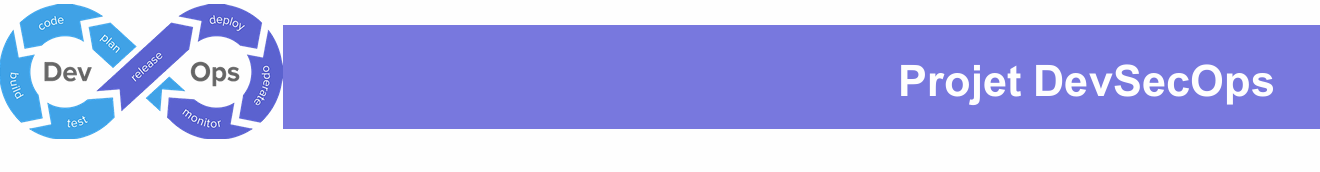
\includegraphics[width=6.5cm]{header-devops.png}
\end{minipage}

\vspace{1.5cm}

{\color{ensablue}\rule{\textwidth}{2pt}}
\vspace{0.8cm}

{\color{ensablue}\LARGE\bfseries RAPPORT TECHNIQUE}\\[0.4cm]
{\color{ensablue}\Large\bfseries Plateforme IntelliOps}\\[0.3cm]
{\color{ensablue}\large Étude des sources et modes de collecte}

\vspace{1.2cm}
{\color{ensablue}\rule{\textwidth}{2pt}}
\vspace{1.2cm}

{\large \textbf{Auteur :} LACHHAB Mohammed}\\[0.4cm]
{\large \textbf{Filière :} GINF2 --- ENSA de Tanger}\\[0.4cm]
{\large \textbf{Année universitaire :} 2025-2026}
\end{center}
\end{titlepage}

\tableofcontents
\newpage

% ===================== SECTION 1 =====================
\section{Synthèse Comparative des Modes de Collecte}

La plateforme IntelliOps repose sur une architecture d'ingestion qui centralise les événements de sécurité et de qualité provenant de sources hétérogènes (GitHub, GitLab CI/CD, Jenkins, SonarQube/SonarCloud, OWASP ZAP, Trivy, Prometheus/Alertmanager, Docker \& Logs Linux, Kubernetes). Avant tout transfert vers l'Agent 1, les événements bruts transitent par un point d'entrée unique :

\begin{center}
\code{POST /internal/agent1/raw-events}
\end{center}

Deux paradigmes d'ingestion coexistent, choisis selon la nature de chaque source.

\subsection{Mode Hybride Push + Pull (Webhook + REST API)}

Ce mode s'applique aux plateformes SaaS ou persistantes qui n'envoient, via leur webhook, que des \emph{métadonnées} (statut, identifiant de build, clé de projet) et non le contenu détaillé des logs ou des vulnérabilités.

\textbf{Déroulement :}
\begin{enumerate}
  \item La source émet un \emph{webhook} (Push) vers un endpoint dédié, par exemple \code{POST /v1/ingest/github}.
  \item Le service d'ingestion vérifie l'authenticité de la requête (signature HMAC ou token d'en-tête) et répond immédiatement \emph{HTTP 200 OK} pour acquitter l'événement sans bloquer l'appelant.
  \item Le service déclenche ensuite un \emph{pull} asynchrone via l'API REST de la source (par exemple \code{GET /repos/{owner}/{repo}/actions/jobs/{job\_id}/logs}) pour récupérer le détail (logs de build, issues, traces).
  \item Les données enrichies sont alors transmises à l'Agent 1 via \code{POST /internal/agent1/raw-events}.
\end{enumerate}

Ce mode est retenu pour \textbf{GitHub Actions}, \textbf{GitLab CI/CD} et \textbf{SonarQube/SonarCloud}.

\subsection{Mode Direct Push (Single-Step)}

Ce mode s'applique aux sources capables d'envoyer, en une seule requête, l'intégralité des métadonnées et des logs/rapports : étapes CI/CD, Alertmanager, ou agents de bord (Edge / in-cluster).

\textbf{Déroulement :}
\begin{enumerate}
  \item Un événement est détecté localement (échec de build, alerte, événement Kubernetes, log critique).
  \item Le client (script CI, agent Vector/FluentBit/k8s-event-exporter) constitue une requête unique contenant métadonnées et payload brut (\emph{raw\_logs}, \emph{zap\_report.json}, rapport Trivy, etc.).
  \item Le client effectue un \emph{POST} direct vers l'endpoint d'ingestion correspondant, authentifié par un token interne (\code{X-IntelliOps-Token} ou Bearer token).
  \item Le service valide et transmet immédiatement à l'Agent 1.
\end{enumerate}

Ce mode est retenu pour \textbf{Jenkins}, \textbf{OWASP ZAP} (option conteneur éphémère), \textbf{Trivy}, \textbf{Prometheus/Alertmanager}, \textbf{Docker \& Logs Linux} et \textbf{Kubernetes}. Il évite d'exposer les serveurs internes à Internet et évite de stocker leurs credentials côté plateforme.

\subsection{Tableau Récapitulatif par Technologie}

\begin{table}[H]
\centering
\small
\begin{tabular}{@{}p{2.6cm}p{2.6cm}p{2.6cm}p{4.6cm}p{3.2cm}@{}}
\toprule
\textbf{Outil} & \textbf{Domaine} & \textbf{Mode de déclenchement} & \textbf{Action de collecte} & \textbf{Authentification} \\
\midrule
GitHub Actions & CI/CD & Webhook (push) + API (pull) & Logs de jobs/workflows \& métadonnées & Fine-grained PAT (HMAC \code{x-hub-signature-256}) \\
GitLab CI/CD & CI/CD & Webhook (push) + API (pull) & Traces de jobs \& métadonnées & PAT (\code{PRIVATE-TOKEN}, \code{X-Gitlab-Token}) \\
Jenkins & CI/CD & Direct push (post \{ failure \}) & Tail des logs console + métadonnées & \code{X-IntelliOps-Token} \\
SonarQube / SonarCloud & Qualité code & Webhook (push) + API Issues (pull) & Vulnérabilités, code smells, bugs & Bearer User Token + HMAC webhook \\
OWASP ZAP & Sécurité applicative & Direct push (conteneur éphémère) ou pull (daemon) & Rapports ZAP JSON (\code{zap\_report.json}) & \code{X-IntelliOps-Token} / API Key ZAP \\
Trivy & Sécurité des images \& IaC & Direct push (CLI / Operator) & Vulnérabilités HIGH/CRITICAL & \code{X-IntelliOps-Token} \\
Prometheus / Alertmanager & Métriques \& alerting & Webhook direct (pull PromQL optionnel) & Alertes groupées \& dédoublonnées & Bearer Project Token \\
Docker \& Logs Linux & Logs hôtes \& conteneurs & Edge shipper (Vector / FluentBit) & Événements Docker, logs stdout/stderr, syslog, journald & \code{POST /v1/ingest/logs} \\
Kubernetes & Orchestration & In-cluster (event-exporter + DaemonSet) & Événements K8s Warning + logs pods & ServiceAccount + RBAC \\
\bottomrule
\end{tabular}
\caption{Synthèse des modes de collecte par source de données.}
\label{tab:synthese}
\end{table}

% ===================== SECTION 2 (9 sources) =====================

\section{Etude Détaillée par Source de Données}

\subsection{GitHub Actions}

\label{subsec:github}
\paragraph{Déclenchement et collecte.} GitHub Actions utilise un \emph{mode hybride Push + Pull}. Le webhook GitHub (\code{push}, \code{pull\_request}, \code{workflow\_run}, \code{check\_run}, etc.) ne transporte que des métadonnées (nom du workflow, statut, identifiant du job, SHA du commit). Dès réception du \code{POST /v1/ingest/github}, le service vérifie la signature HMAC \code{x-hub-signature-256} calculée avec le \emph{webhook secret}, répond immédiatement \emph{HTTP 200 OK}, puis effectue un \emph{pull} asynchrone via l'API GitHub pour récupérer le détail des logs :

\begin{lstlisting}[caption={Appel API REST GitHub pour récupérer les logs d'un job}]
GET /repos/{owner}/{repo}/actions/jobs/{job_id}/logs
Authorization: Bearer <PAT Fine-grained>
\end{lstlisting}

\paragraph{Authentification et base de données.} L'authentification repose sur un \emph{Fine-grained PAT} avec le scope \code{Actions: Read-only}. Ce PAT est stocké chiffré en base, associé au mapping dépôt/platforme, ainsi que le \emph{webhook secret} utilisé pour vérifier l'integrité des requêtes entrantes.

\begin{figure}[H]
\centering
\includegraphics[width=\textwidth]{github.png}
\caption{Séquence de collecte GitHub Actions.}
\end{figure}

\subsection{GitLab CI/CD}

\label{subsec:gitlab}
\paragraph{Déclenchement et collecte.} Comme GitHub, GitLab CI/CD utilise un \emph{mode hybride Push + Pull}. Le webhook GitLab (\code{push}, \code{merge request}, \code{pipeline}, \code{job}) ne transmet que des métadonnées. Le service écoute sur \code{POST /v1/ingest/gitlab} et vérifie l'en-tête \code{X-Gitlab-Token} contre le token configuré côté IntelliOps, puis répond \emph{HTTP 200 OK}. Un pull asynchrone récupère ensuite la trace complète du job :

\begin{lstlisting}[caption={Appel API REST GitLab pour récupérer la trace d'un job}]
GET /api/v4/projects/{project_id}/jobs/{job_id}/trace
PRIVATE-TOKEN: <PAT>
\end{lstlisting}

\paragraph{Authentification et base de données.} L'authentification utilise un \emph{PAT} passé en en-tête \code{PRIVATE-TOKEN} avec le scope \code{read\_api}. GitLab SaaS et GitLab Self-Managed sont supportés via une \emph{base URL} dynamique stockée en base. Les champs persistés sont : PAT chiffré, \code{PRIVATE-TOKEN}, \code{X-Gitlab-Token}, URL de base, mapping projet, et secret de webhook.

\begin{figure}[H]
\centering
\includegraphics[width=\textwidth]{gitlab_cicd.png}
\caption{Séquence de collecte GitLab CI/CD.}
\end{figure}

\subsection{Jenkins}

\label{subsec:jenkins}
\paragraph{Pourquoi un Direct Push en une étape.} Jenkins est typiquement déployé en interne et n'est pas exposé sur Internet. Un mode hybride webhook + pull exigerait soit d'exposer Jenkins aux appels entrants, soit de stocker les credentials Jenkins (utilisateur/mot de passe ou token API) côté plateforme pour poller l'API Jenkins. Le \emph{Direct Push} en une étape élimine ces deux contraintes : le serveur Jenkins initie lui-même la requête sortante, aucune credential Jenkins n'est stockée par IntelliOps, et le périmètre d'exposition réseau est nul.

\paragraph{Fonctionnement.} Dans le \code{Jenkinsfile}, le bloc \code{post \{ failure \}} intercepte l'échec d'un build. Il extrait la \emph{queue} de la console via \code{currentBuild.rawBuild.getLog(150)} (les 150 dernières lignes) afin d'éviter des payloads trop volumineux susceptibles de provoquer des timeouts. Les métadonnées (nom du job, numéro de build, statut, URL) et les \code{raw\_logs} sont envoyés dans une seule requête \code{POST /v1/ingest/jenkins}, authentifiée par l'en-tête \code{X-IntelliOps-Token}.

\begin{lstlisting}[caption={Jenkinsfile - bloc post d'envoi direct vers IntelliOps}]
pipeline {
    agent any
    stages {
        stage('Build') { steps { sh 'make build' } }
        stage('Test')  { steps { sh 'make test' } }
    }
    post {
        failure {
            script {
                def logs = currentBuild.rawBuild.getLog(150)
                def payload = [
                    job: env.JOB_NAME,
                    build: env.BUILD_NUMBER,
                    status: 'FAILURE',
                    url: env.BUILD_URL,
                    raw_logs: logs
                ]
                def json = groovy.json.JsonOutput.toJson(payload)
                sh "curl -X POST https://intelliops.local/v1/ingress/jenkins " +
                   "-H 'X-IntelliOps-Token: \$INTELLIOPS_TOKEN' " +
                   "-H 'Content-Type: application/json' " +
                   "-d '${json}'"
            }
        }
    }
}
\end{lstlisting}

\begin{figure}[H]
\centering
\includegraphics[width=\textwidth]{jenkins.png}
\caption{Séquence de collecte Jenkins.}
\end{figure}

\subsection{SonarQube Server et SonarCloud}

\label{subsec:sonar}
\paragraph{Pourquoi un Push + Pull en deux étapes.} Le webhook SonarQube ne transporte que le statut du \emph{Quality Gate} (pass/fail) et des métadonnées de projet ; il ne contient ni les vulnérabilités, ni les code smells, ni les bugs avec leur fichier et leur ligne. Une collecte en deux étapes est donc indispensable : le webhook signale l'événement (Phase 1), puis une requête API récupère les détails des issues (Phase 2).

\paragraph{Phase 1 - Webhook du Quality Gate.} Lorsque le statut du Quality Gate passe à \code{ERROR}, SonarQube/SonorCloud POSTe un webhook signé \code{X-Sonar-Webhook-HMAC-SHA256}. Le service vérifie la signature et répond \emph{HTTP 200 OK}.

\paragraph{Phase 2 - Pull des issues via API REST.} Le service appelle ensuite l'endpoint de recherche d'issues non résolues :

\begin{lstlisting}[caption={Appel API SonarQube/SonorCloud pour récupérer les issues}]
GET {base_url}/api/issues/search?componentKeys={projectKey}&resolved=false
Authorization: Bearer <User Token>
\end{lstlisting}

\paragraph{Option 1 : SonarCloud (SaaS).} \code{base_url} = \code{https://sonarcloud.io}. Pas d'hébergement à gérer, authentification par Bearer User Token SonarCloud.

\paragraph{Option 2 : SonarQube Self-Hosted.} \code{base_url} est l'URL de l'instance propre à l'organisation (ex. \code{https://sonar.internal.company}). Le même handler unifié est utilisé, le \code{base_url} étant dynamique selon l'édition déclarée en base.

\paragraph{Champs de la base de données (unifiés).}

\begin{table}[H]
\centering
\small
\begin{tabular}{@{}p{3.2cm}p{8.2cm}@{}}
\toprule
\textbf{Champ} & \textbf{Description} \\
\midrule
\code{edition\_type} & \code{SAAS} (SonarCloud) ou \code{SELF\_HOSTED} (SonarQube) \\
\code{base\_url} & URL de base de l'instance (\code{https://sonarcloud.io} ou URL propre) \\
\code{project\_key} & Clé du projet Sonar (\code{componentKeys}) \\
\code{auth\_token} & Bearer User Token (chiffré) pour l'API \code{/api/issues/search} \\
\code{webhook\_secret} & Secret utilisé pour vérifier \code{X-Sonar-Webhook-HMAC-SHA256} \\
\bottomrule
\end{tabular}
\caption{Champs unifiés de la base de données pour SonarQube / SonarCloud.}
\label{tab:sonar-db}
\end{table}

\begin{figure}[H]
\centering
\includegraphics[width=\textwidth]{sonarQube.png}
\caption{Séquence de collecte SonarQube / SonarCloud.}
\end{figure}

\subsection{OWASP ZAP}

\label{subsec:zap}
\paragraph{Les trois cas de scan supportés.}
\begin{itemize}
  \item \textbf{Cas A} (\code{zap-baseline.py}) : scan de base d'une application web cible, sans fichier de définition d'API.
  \item \textbf{Cas B} (\code{zap-api-scan.py}) : scan d'API à partir d'une définition OpenAPI / Swagger / GraphQL.
  \item \textbf{Cas C} (\code{zap-full-scan.py}) : scan complet (spider + active scan) d'une application.
\end{itemize}

\paragraph{Deux architectures de collecte.}
\begin{itemize}
  \item \textbf{Option 1 - Conteneur CI/CD éphémère (Direct Push).} Le conteneur ZAP exécute le scan, produit \code{zap\_report.json}, puis l'envoie en une seule requête \code{POST} authentifiée par \code{X-IntelliOps-Token} avec l'option \code{-I} (rapport JSON).
  \item \textbf{Option 2 - Daemon ZAP persistant (Pull).} Une instance ZAP persistante expose son API locale ; le service d'ingestion interroge l'API ZAP pour récupérer le rapport.
\end{itemize}

\paragraph{Filtrage du bruit.} Avant la remise à l'Agent 1, les alertes de niveau \code{riskcode "0"} (Informational) sont filtrées pour ne conserver que les incidents pertinents.

\begin{lstlisting}[caption={Scan ZAP baseline en CI et envoi direct}]
docker run -t owasp/zap2docker-stable zap-baseline.py \
    -t https://app.example.com -I -z "-config.api.disablekey=true" \
    -w /zap/wrk/
cat /zap/wrk/zap_report.json | curl -X POST https://intelliops.local/v1/ingest/zap \
    -H 'X-IntelliOps-Token: $INTELLIOPS_TOKEN' \
    -H 'Content-Type: application/json' --data-binary @-
\end{lstlisting}

\begin{figure}[H]
\centering
\includegraphics[width=\textwidth]{ZAP.png}
\caption{Séquence de collecte OWASP ZAP.}
\end{figure}

\subsection{Trivy}

\label{subsec:trivy}
\paragraph{Les trois cas de scan.}
\begin{itemize}
  \item \textbf{Cas A} (\code{trivy image}) : analyse d'images conteneurs pour les vulnérabilités OS et dépendances applicatives.
  \item \textbf{Cas B} (\code{trivy fs}) : analyse du système de fichiers et des fichiers de verrouillage (lockfiles) des dépendances.
  \item \textbf{Cas C} (\code{trivy config} / \code{trivy k8s}) : analyse de configuration des manifests Terraform, Ansible et Kubernetes.
\end{itemize}

\paragraph{Environnements d'exécution.} Trivy s'exécute soit en CLI éphémère dans le pipeline CI/CD, soit via l'opérateur Trivy dans Kubernetes.

\paragraph{Flux Direct Push.} Le scan génère un rapport JSON qui est filtré pour ne conserver que les sévérités \code{HIGH} et \code{CRITICAL}, puis envoyé en une seule requête \code{POST /v1/ingest/trivy} authentifiée par \code{X-IntelliOps-Token}.

\begin{lstlisting}[caption={Scan Trivy image et envoi direct des vulnérabilités critiques}]
trivy image --format json --severity HIGH,CRITICAL \
    --output trivy_report.json registry.example.com/app:latest
curl -X POST https://intelliops.local/v1/ingest/trivy \
    -H 'X-IntelliOps-Token: $INTELLIOPS_TOKEN' \
    -H 'Content-Type: application/json' --data-binary @trivy_report.json
\end{lstlisting}

\begin{figure}[H]
\centering
\includegraphics[width=\textwidth]{trivy.png}
\caption{Séquence de collecte Trivy.}
\end{figure}

\subsection{Prometheus et Alertmanager}

\label{subsec:prometheus}
\paragraph{Pas de flux continu de séries temporelles.} Les séries temporelles brutes (métriques toutes les 15 s) ne sont pas streamées : le volume serait trop important et l'information de sécurité n'est pas dans la métrique brute mais dans l' \emph{alerte} qui en découle.

\paragraph{Les trois cas de métriques surveillées.}
\begin{itemize}
  \item \textbf{Cas A} : hôte / VM via \emph{Node Exporter} (CPU, mémoire, disque, réseau).
  \item \textbf{Cas B} : conteneurs / Kubernetes via \emph{cAdvisor} et \emph{kube-state-metrics}.
  \item \textbf{Cas C} : applications / APIs via leurs exporters dédiés.
\end{itemize}

\paragraph{Évaluation PromQL et Alertmanager.} Prometheus évalue les règles PromQL et génère des alertes. Alertmanager assure le \emph{grouping} et la \emph{déduplication} (\code{group\_by}) avant de notifier IntelliOps.

\paragraph{Collecte.} Une \emph{Single-Step Direct Webhook Push} est utilisée : Alertmanager POSTe l'alerte groupée vers \code{POST /v1/ingest/prometheus}, authentifiée par un \emph{Bearer Project Token}. Un \emph{pull PromQL optionnel} permet d'enrichir l'alerte avec le contexte des métriques au moment de l'incident.

\begin{lstlisting}[caption={alertmanager.yml - envoi direct vers IntelliOps}]
route:
  group_by: ['alertname', 'cluster', 'service']
  group_wait: 30s
  group_interval: 5m
  receiver: 'intelliops'
receivers:
  - name: 'intelliops'
    webhook_configs:
      - url: 'https://intelliops.local/v1/ingest/prometheus'
        http_config:
          bearer_token: <PROJECT_TOKEN>
\end{lstlisting}

\begin{figure}[H]
\centering
\includegraphics[width=\textwidth]{prometheus.png}
\caption{Séquence de collecte Prometheus / Alertmanager.}
\end{figure}

\subsection{Docker et Logs Linux}

\label{subsec:docker}
\paragraph{Les trois cas cibles sur l'hôte.}
\begin{itemize}
  \item \textbf{Cas A} : événements Docker Engine via \code{/var/run/docker.sock} (\code{oom} / \code{OOMKilled}, \code{die}, boucles de redémarrage).
  \item \textbf{Cas B} : logs \code{stdout}/\code{stderr} des conteneurs.
  \item \textbf{Cas C} : logs Linux système (\code{/var/log/syslog}, \code{/var/log/auth.log}, \code{journald}).
\end{itemize}

\paragraph{Filtrage en bordure (Edge).} Un shipper léger (\textbf{Vector} ou \textbf{FluentBit}) tourne sur l'hôte, supprime localement le bruit (\code{INFO}/\code{DEBUG}) et ne pousse que les incidents critiques vers \code{POST /v1/ingest/logs}.

\begin{lstlisting}[caption={vector.yaml - collecte logs et événements Docker, filtrage bruit}]
sources:
  docker_events:
    type: docker_socket
    endpoint: /var/run/docker.sock
  container_logs:
    type: file
    include: ['/var/log/containers/*.log']
  syslog:
    type: file
    include: ['/var/log/syslog', '/var/log/auth.log']

transforms:
  filter_noise:
    type: filter
    condition: | 
      .level != "INFO" and .level != "DEBUG"

sinks:
  intelliops:
    type: http
    inputs: ["docker_events", "container_logs", "syslog", "filter_noise"]
    endpoint: https://intelliops.local/v1/ingest/logs
    headers:
      X-IntelliOps-Token: "${INTELLIOPS_TOKEN}"
    encoding: json
\end{lstlisting}

\begin{figure}[H]
\centering
\includegraphics[width=\textwidth]{docker_linux.png}
\caption{Séquence de collecte Docker et logs Linux.}
\end{figure}

\subsection{Kubernetes}

\label{subsec:k8s}
\paragraph{Les trois cas cibles.}
\begin{itemize}
  \item \textbf{Cas A} : échecs du cycle de vie Pod/Conteneur via l'API Événements Kubernetes (\code{CrashLoopBackOff}, \code{ImagePullBackOff}, \code{OOMKilled}, \code{FailedScheduling}).
  \item \textbf{Cas B} : alertes de santé des nodes (\code{NodeNotReady}, \code{DiskPressure}, \code{MemoryPressure}).
  \item \textbf{Cas C} : logs des pods de microservice en échec.
\end{itemize}

\paragraph{Architecture in-cluster.} Un \code{kubernetes-event-exporter} (\emph{Déploiement}) capture les événements du cluster, couplé à un \emph{DaemonSet} Vector/FluentBit pour les logs des pods. L'authentification s'appuie sur un \emph{ServiceAccount} Kubernetes avec les \emph{RBAC} nécessaires (lecture des \code{events}, \code{pods}, \code{nodes}).

\paragraph{Filtrage.} Les événements de niveau \code{Normal} sont filtrés localement ; seuls les événements \code{Warning} sont poussés vers \code{POST /v1/ingest/k8s}.

\begin{lstlisting}[caption={ConfigMap - filtrage et routage des événements Kubernetes vers IntelliOps}]
apiVersion: v1
kind: ConfigMap
metadata:
  name: intelliops-k8s-collector
  namespace: intelliops
data:
  config.yaml: |
    sources:
      k8s_events:
        type: kubernetes_events
    transforms:
      keep_warnings:
        type: filter
        condition: | .reason != "Normal"
    sinks:
      intelliops:
        type: http
        inputs: ["k8s_events", "keep_warnings"]
        endpoint: https://intelliops.local/v1/ingest/k8s
        headers:
          X-IntelliOps-Token: "${INTELLIOPS_TOKEN}"
        encoding: json
\end{lstlisting}

\begin{figure}[H]
\centering
\includegraphics[width=\textwidth]{kubernetes.png}
\caption{Séquence de collecte Kubernetes.}
\end{figure}

\end{document}
